\documentclass[conference]{IEEEtran}
\IEEEoverridecommandlockouts
% The preceding line is only needed to identify funding in the first footnote. If that is unneeded, please comment it out.
\usepackage[left=1.62cm,right=1.62cm,top=1.9cm,bottom=4.4cm]{geometry}
\setlength{\columnsep}{0.25in}
\usepackage{cite}
\usepackage{algorithmic}
\usepackage{graphicx}
\usepackage{textcomp}
\usepackage{xcolor}
\usepackage{natbib}
\usepackage{booktabs}
\usepackage{amsmath,amssymb,amsfonts}
\usepackage{CJK}
\usepackage{CJKutf8}
\usepackage{pinyin}
\bibpunct{[}{]}{;}{a}{,}{,}




\def\BibTeX{{\rm B\kern-.05em{\sc i\kern-.025em b}\kern-.08em
    T\kern-.1667em\lower.7ex\hbox{E}\kern-.125emX}}
\begin{document}
\begin{CJK*}{UTF8}{gbsn}%{bsmi}

\title{Quantitative Evaluation of Translation Quality and Computational Efficiency in Semantic vs. Phonetic Strategies for Chinese Scientific Terms\\
%Character and Component Threshold Determination in Chinese, Japanese, and Korean Hanzi Image Recognition\\
%Quantitative Analysis of Translation Quality and Computational Cost in Semantic and Phonetic Translation of Chinese Scientific Terms


\thanks{This work has been partially supported by the Brazilian National Council for Scientific and Technological Development (CNPq) under the grant number 309545/2021-8.
}
}

%Names
\author{\IEEEauthorblockN{Li Weigang}
\IEEEauthorblockA{\textit{Computer Science Department} \\
\textit{University of  Brasilia}\\
Brasília, Brazil \\
weigang@unb.br}
\and


\IEEEauthorblockN{Pedro Carvalho Brom}
\IEEEauthorblockA{\textit{Mathematics Department} \\
\textit{Federal Institute of Brasilia}\\
Brasília, Brazil \\
pedro.brom@ifb.edu.br}
\and
\IEEEauthorblockN{Rafael Marconi Ramos}
\IEEEauthorblockA{\textit{Computer Science Department} \\
\textit{University of  Brasilia}\\
Brasília, Brazil \\
rafaelmr@gmail.com}


}

\maketitle

\begin{abstract}
This study presents a quantitative evaluation of translation quality and computational efficiency between semantic and phonetic translation strategies for Chinese scientific terms, using Large Language Models (LLMs). Focusing on two representative domains—the Chinese periodic table and heterocyclic compound nomenclature—we propose a back-translation framework (LLM-BT) specifically designed for evaluating scientific terminology translation, conducting Chinese→English→Chinese cycles with Grok, DeepSeek, and GPT-4 models. BLEU scores are used to assess translation accuracy. Results show that semantic translation of element names achieves near-perfect performance (BLEU ≈ 1.00), leveraging the compositional properties of Chinese characters. In contrast, phonetic translation of heterocyclic compounds yields lower BLEU scores (0.55–0.65), reflecting the inherent challenges of transliteration. Multilingual comparisons using Google Translate (Chinese, Japanese, Korean, English) further validate the superiority of semantic translation strategies (BLEU 0.94–0.99) over phonetic approaches (0.16–0.36). Also, byte-level analysis reveals that Chinese semantic and pictophonetic names are more compact (3 bytes per element) compared to Japanese (13.73 bytes) and Korean (8.97 bytes) transliterations. These findings highlight the dual advantages of semantic translation for both accuracy and computational efficiency. We advocate prioritizing semantic strategies in scientific terminology standardization and cross-linguistic knowledge transfer.
%This study presents a quantitative evaluation of translation quality and computational efficiency between semantic and phonetic translation strategies for Chinese scientific terms, using Large Language Models (LLMs). Focusing on two representative domains—the Chinese periodic table of elements and heterocyclic compound nomenclature—we adopt a back-translation framework (LLM-BT), involving Chinese → English → Chinese translation cycles with LLMs such as Grok, DeepSeek, and GPT-4. BLEU scores are used to assess translation fidelity. Results show that semantic translations of element names achieve near-perfect accuracy (BLEU ≈ 1.00), leveraging the generative and compositional properties of Chinese characters. In contrast, phonetic translations for heterocyclic compounds yield lower scores (BLEU 0.55–0.65), reflecting the inherent challenges of transliteration. Multilingual comparisons using Google Translate across Chinese, Japanese, Korean, and English further validate the superiority of semantic translation strategies (BLEU 0.94–0.99) over phonetic approaches (BLEU 0.16–0.36). Additionally, byte-level analysis reveals that Chinese semantic and pictophonetic names are significantly more compact (3 bytes per element) compared to Japanese (13.73 bytes) and Korean (8.97 bytes) transliterations. These findings highlight the dual benefits of semantic translation in improving both translation accuracy and computational efficiency for Chinese NLP tasks. We advocate for prioritizing semantic strategies in scientific terminology standardization and cross-linguistic information transfer, offering new insights for optimizing LLM performance on domain-specific translation tasks.

%This study quantitatively evaluates the translation quality and computational cost of semantic and phonetic strategies in Chinese scientific terminology using large language models (LLMs). Focusing on the Chinese periodic table and heterocyclic compounds, we employ a back-translation framework, LLM-BT, (eg. Chinese → English → Chinese) with LLMs such as Grok, DeepSeek, and GPT-4, assessing results using BLEU scores. Semantic translation of element names achieves near-perfect accuracy (BLEU 1.00), leveraging the generative properties of Chinese characters, while phonetic translation of heterocyclic compound names yields lower scores (BLEU 0.55–0.65), reflecting the challenges of transliteration. Multilingual comparisons (Chinese, Japanese, Korean, English) via Google Translate further confirm the superiority of semantic translation (BLEU 0.94–0.99) over phonetic translation (BLEU 0.16–0.36). Byte analysis reveals that Chinese pictophonetic and semantic names are more compact (3 bytes per element) than Japanese (13.73 bytes per element) or Korean (8.97 bytes per element) transliterations. These findings highlight the advantages of semantic strategies for both translation accuracy and computational efficiency in Chinese NLP. We advocate prioritizing semantic translation to improve terminology standardization and cross-linguistic transferability, offering insights for optimizing scientific nomenclature and LLM performance.
\end{abstract}

\begin{IEEEkeywords}
Back-translation, CNLP, Semantic generative, LLM-BT, Semantic and Phonetic Translation, Scientific Terms.
\end{IEEEkeywords}

\section{INTRODUCTION}

The rapid advancement of large language models (LLMs) like Grok, DeepSeek, and ChatGPT has enhanced text generation, offering new insights into Chinese language properties \citep{chang2024survey,weigang2024six,pham2025top}. Unlike phonetic languages (e.g., English, Portuguese), where chemical element names average 7.82 letters (max 13, e.g., Rutherfordium), Chinese uses a single character per element (e.g., “氢” for hydrogen), encoded in 3 bytes via Unicode/UTF-8. This compactness, rooted in the pictophonetic structure from “Shuowen Jiezi-说文解字” (c. 100 AD), integrates semantic richness—e.g., “氢” implies gaseous lightness—outperforming Japanese (13.73 bytes) and Korean (8.97 bytes) transliterations (see Fig. \ref{fig:four elements}).
%The rapid advancement of large language models (LLMs) has significantly enhanced artificial intelligence capabilities in text generation, offering new opportunities to explore the unique generative properties of the Chinese language \citep{chang2024survey,weigang2024six,pham2025top}. Unlike phonetic languages such as English or Portuguese, where scientific terms like chemical element names average 7.82 letters (e.g., Rutherfordium “\begin{CJK}{UTF8}{bsmi}鑪"\end{CJK} with 13 letters maximum), Chinese represents each of the 118 periodic table elements with a single character, requiring only 3 bytes in Unicode/UTF-8 encoding. This compactness, rooted in the pictophonetic structure of Chinese characters, dates back nearly two thousand years to “Shuowen Jiezi-说文解字", which systematized character formation—offering insights still valuable for modern natural language processing (NLP). For example, the character “氢" (hydrogen) not only denotes a chemical element but also implies its gaseous, lightweight nature, demonstrating how Chinese integrates semantic richness with brevity, a feature less evident in Japanese (13.73 bytes per element) or Korean (8.97 bytes per element) transliterations, see Fig. \ref{fig:four elements}.


\begin{figure}[h!]
    \centering
    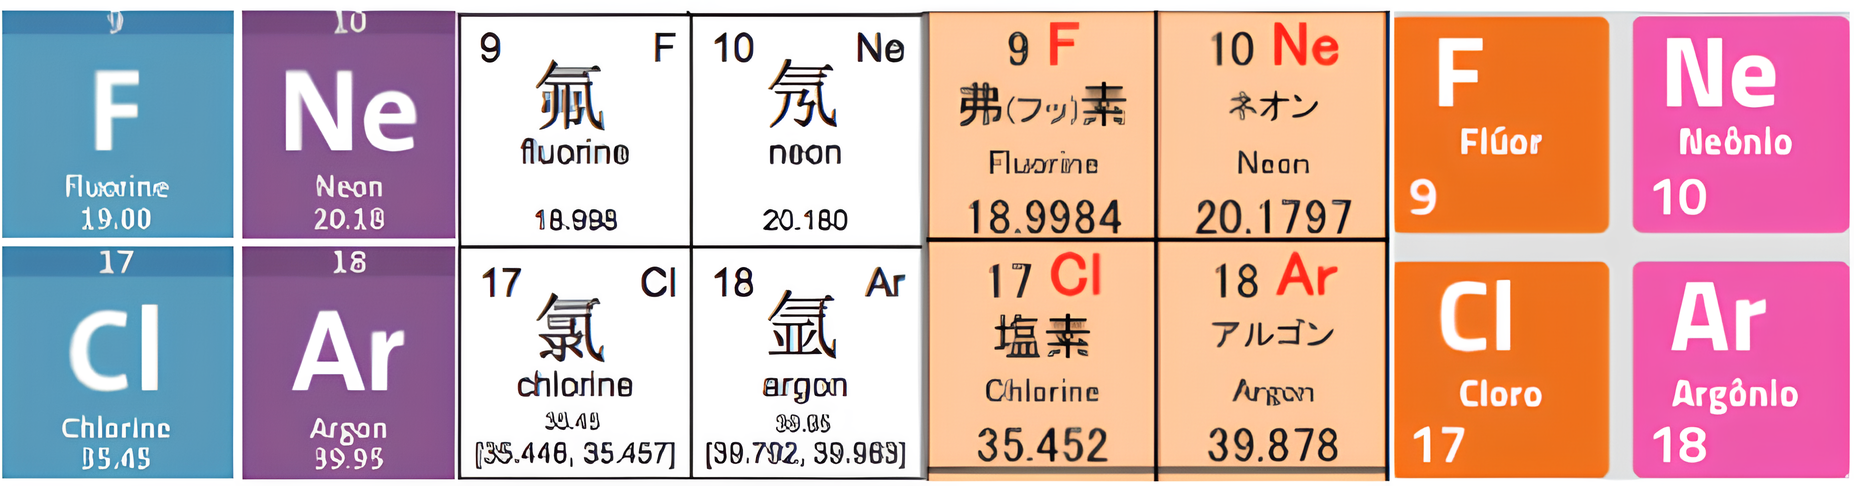
\includegraphics[width = 0.48\textwidth]{img/Four elements 2.png}
    \caption{Examples of four elements (fluorine, neon, chlorine, and argon) from the periodic tables of English, Chinese, Japanese, and Portuguese.}
    \label{fig:four elements}
\end{figure}

%This efficiency extends beyond elements to the naming of chemical compounds, guided by efforts like the "Nomenclature of Organic Compounds-2017"  from the Chinese Chemical Society \citep{ccs2017nomenclature}, which emphasizes systematization and standardization. While semantic translation excels in element naming—e.g., “烃" (hydrocarbon) combines “碳" (carbon) and “氢" (hydrogen) with a “火" (fire) radical to reflect combustion—organic compound naming often relies on phonetic transliteration, especially for heterocyclic compounds. Historical debates were recorded by \citep{hejuan2019nomencl}, highlighting the ongoing tension in chemical nomenclature. Phonetic names like dithiadiazole, transliterated using mouth-radical characters (e.g., “二噻二唑”), have been criticized as “gibberish” for lacking intrinsic meaning and hindering comprehension, yet their complexity sometimes warrants simplification. This phonetic approach deviates from the International Union of Pure and Applied Chemistry (IUPAC) standards \citep{favre2014nomenclature} and increases computational cost, diminishing the efficiency observed in element naming. In this study, we selected specific expert comments and key excerpts from \citep{hejuan2019nomencl}, referring to them as “Xue Dejiong’s Dilemma” for analytical purposes.

%Analyzing the nomenclature of the periodic table and heterocyclic organic compounds reveals how language choice influences term comprehension and efficiency in multilingual contexts. While English and Portuguese translations of the periodic table are relatively straightforward, early Japanese transliterations led to confusion due to inconsistent character usage. In contrast, the Chinese system utilizes pictophonetic characters—such as “砹" (astatine), where the radical “石" (stone) indicates non-metallic properties—enhancing both human readability and machine processing. However, phonetic transliterations of complex compounds (e.g., bisbenzyltetrahydroisoquinolines as “双苄基四氢异喹啉类") exhibit lower translation accuracy and efficiency, posing challenges for cross-linguistic understanding.

%This study quantitatively examines these differences using LLMs like Grok, DeepSeek, and ChatGPT through a back-translation framework \citep{hoang2018iterative} (Chinese → English → Chinese), focusing on translation quality (BLEU scores) and computational cost (byte usage). Using the Chinese periodic table and organic compound nomenclature as case studies, we compare semantic and phonetic strategies across Chinese, Japanese, Korean, and Western languages. The main contributions of this study are as follows:
%(1) Proposing a systematic LLM-BT-based evaluation framework for scientific terminology translation;
%(2) Conducting quantitative comparisons across semantic and phonetic translation strategies;
%(3) Introducing byte-level analysis to assess computational efficiency in multilingual contexts.
%The findings advocate for semantic translation to improve term comprehensibility, cross-linguistic transferability, and efficiency in Chinese NLP (CNLP), addressing gaps left by prior qualitative studies.

%While scientific terminology translation has been qualitatively analyzed, a comprehensive quantitative framework is still lacking. This study fills this gap by applying statistical methods, including non-parametric BLEU analysis and computational cost evaluation using Unicode/UTF-8 byte representation. By systematically comparing semantic and phonetic translation strategies across LLMs, our approach establishes a reproducible framework for assessing cross-linguistic transferability and computational efficiency in scientific naming conventions.

This efficiency extends to compound naming, guided by the Chinese Chemical Society’s “Nomenclature of Organic Compounds-2017” \citep{ccs2017nomenclature}. Semantic translation excels for elements (e.g., “烃” for hydrocarbon), but phonetic transliteration dominates complex compounds (e.g., dithiadiazole as “二噻二唑”), often criticized as unintelligible \citep{hejuan2019nomencl}. This deviates from International Union of Pure and Applied Chemistry (IUPAC) standards \citep{favre2014nomenclature}, increasing computational cost. We term this trade-off “Xue Dejiong’s Dilemma” based on expert insights from \citep{hejuan2019nomencl}.

This study quantitatively compares semantic and phonetic strategies using an LLM back-translation framework, LLM-BT (e.g., Chinese → English → Chinese) \citep{hoang2018iterative}, assessing translation quality (BLEU scores) and byte efficiency. Case studies include the Chinese periodic table and organic compounds across Chinese, Japanese, Korean, and Western languages. Contributions include: (a) Proposing a systematic LLM-BT-based evaluation framework for scientific terminology translation; (b) Conducting quantitative comparisons across semantic and phonetic translation strategies; (c) Introducing byte-level analysis to assess computational efficiency in multilingual contexts. Results advocate semantic translation for improved comprehensibility and efficiency in Chinese NLP (CNLP), addressing gaps in prior qualitative research.

\section{Basic Corpus}

\subsection{Periodic Table Corpus}

This study constructs a multilingual element name corpus based on the Periodic Table of Elements. The corpus covers six languages, including English (PT-EN118), Russian (PT-RU118), Portuguese (PT-PT118), Latin (PT-LA118), Chinese (PT-ZH118), Japanese (PT-JA118), and Korean (PT-KO118), totaling 118 element names. Among them, Korean element names are derived from phonetic transliteration of English, while Chinese element names follow pictophonetic and semantic translation from English. Japanese element naming is more complex, incorporating three forms: Kanji (semantic translation), Kanji + Kana (semantic + phonetic transliteration), and Pure Kana (phonetic transliteration).
%Due to significant differences in element naming conventions across languages, this study collects Periodic Table corpora in these six languages to analyze translation strategies and linguistic characteristics.

\subsection{Heterocyclic Organic Compound Naming Corpus}
According to the “Principles of Organic Compound Nomenclature - 2017" \citep{ccs2017nomenclature}, Chinese organic compound names generally follow three strategies: semantic translation (based on chemical structure or function), phonetic transliteration (directly reflecting English pronunciation), and conventional usage (adopting established chemical naming traditions or commonly used terms). For more complex compounds, a combination of these strategies may be applied.

Notably, Chapter 8: Natural Products \citep{ccs2017nomenclature} differs from other chapters in two key aspects: (a) Most compound names are transliterations using Chinese characters, in contrast to the more common semantic translation approach. (b) Nearly every compound name is accompanied by its original English name, providing additional clarification.

Based on these characteristics, this study selects 58 heterocyclic organic compound names from Chapter 8, constructing two corpora: Simplified Chinese (HO-ZH58) and English (HO-EN58). These corpora serve as representative data for phonetic transliteration in scientific terminology, facilitating an in-depth analysis of the role of phonetic transliteration in Chinese scientific nomenclature.

\subsection{“Xue Dejiong ’s Dilemma" Corpus}
The debate over whether Chinese names for heterocyclic organic compounds should be semantically translated or phonetically transliterated has been ongoing in the academic community. He Juan conducted a retrospective analysis of this issue \citep{hejuan2019nomencl}. Building on this work, our study curates and extracts relevant statements from chemist Xue Dejiong, forming the “Xue Dejiong’s Dilemma” corpus. This text poses unique linguistic challenges, blending technical, cultural, and rhetorical elements, making it an ideal benchmark for evaluating machine translation performance.

%\subsection{Scientific and technical literature corpus}
%This study collects scientific journal metadata from the overseas edition of CNKI (oversea.cnki.net), including fields such as journal names, article titles, authors, keywords, abstracts, volume numbers, and page numbers. A general scientific corpus is constructed based on ten key scientific disciplines, which include: Chemistry, Biotechnology, Nanotechnology, Telemedicine, Artificial Intelligence, Data Science, Digital Economy, Linguistics, Sociology, Distance Education.

%During data collection, 295 Chinese scientific articles were selected from each discipline, with titles, keywords, and abstracts extracted. The compiled corpus is uploaded to GitHub for further research use. The order of disciplines roughly follows the increasing complexity of language processing. In subsequent linguistic analysis, each category maintains 295 samples, ensuring statistical significance in the study's results.

\section{Statistical Analysis of Computational Cost for Language Processing}

Chinese chemical nomenclature (e.g., elements and compounds) employs semantic and phonetic transcription. This study quantifies their effects using Unicode/UTF-8 encoding, where fewer bytes reflect efficient processing and better nomenclature, while more bytes indicate inefficiency.

\begin{table*}[h!]
\centering
\caption{Comparison of Representation Indicators for Periodic Table Names in Several Languages}
\begin{tabular}{cccccc}
\hline
 & \textbf{Minimum letters} & \textbf{Maximum letters} & \textbf{Average letters} & \textbf{Average bytes} & \textbf{Byte ratio} \\ 
 & \textbf{最少字符} & \textbf{最多字符} & \textbf{平均字符} & \textbf{平均字节(UTF-8)} & \textbf{英语字节比} \\ \hline
\textbf{English 英文} & 3 & 13 & 7.82 & 7.82 & 1 \\ 
\textbf{Latin 拉丁文} & 4 & 13 & 8.07 & 8.07 & 1.05 \\ 
\textbf{Portuguese 葡萄牙文} & 4 & 12 & 7.05 & 7.27 & 0.96 \\ 
\textbf{Russian 俄文} & 3 & 11 & 6.66 & 13.32 & 1.70 \\ 
\textbf{Japanese 日文} & 1 & 9 & 4.58 & 13.73 & 1.76 \\ 
\textbf{Korean 韩文} & 1 & 8 & 2.99 & 8.97 & 1.15 \\ 
\textbf{Chinese 中文} & 1 & 1 & 1 & 3 & 0.38 \\ \hline
%\textbf{SWPC} & 4 & 8 & 4.75 & 4.75 & 0.61 \\ \hline
\end{tabular}
\label{tab:letter_byte_comparison}
\end{table*}

\begin{table*}[htbp]
\centering
\caption{Comparison of Representation Indicators for Phonetically Transcribed Organic Compound Names}
\label{tab:comparison}
\begin{tabular}{cccccc}
\hline
\textbf{Language} & \textbf{Minimum letters} & \textbf{Maximum letters} & \textbf{Average letters} & \textbf{Average bytes} & \textbf{Byte ratio} \\
\textbf{语言} & \textbf{最少字符} & \textbf{最多字符} & \textbf{平均字符} & \textbf{平均字节(UTF-8)} & \textbf{英语字节比} \\
\hline
English 英文 & 9 & 35 & 13.67 & 13.67 & 1 \\

Japanese 日文 & 4 & 18 & 6.43 & 19.34 & 1.41 \\

Korean 韩文 & 2 & 17 & 5.05 & 15.16 & 1.11 \\

Chinese 中文 & 3 & 12 & 6 & 18 & 1.32 \\
\hline
\end{tabular}
\end{table*}

For comparative analysis, English serves as the baseline. The ratio $\gamma$ (gamma) compares element or compound nomenclature in a given language to English. If the representation number is the number of bytes $N_{L,\text{byte}}$, then $\gamma$ is the byte ratio relative to English:

%If the representation number is the number of characters $N_{L,\text{char}}$, then $\gamma$ is the character ratio relative to English:
%\begin{equation}
%\gamma_{\text{char}} = \frac{N_{L,\text{char}}}{N_{\text{Eng},\text{char}}}
%\label{eq:char_ratio}
%\end{equation}

\begin{equation}
\gamma_{\text{byte}} = \frac{N_{L,\text{byte}}}{N_{\text{Eng},\text{byte}}}
\label{eq:byte_ratio}
\end{equation}


\subsection{Comparative Analysis of Multilingual Nomenclature in the Periodic Table}
Statistical data in Table \ref{tab:letter_byte_comparison} shows that the average length of 118 English element names in the Periodic Table is 7.82 letters (7.82 bytes in UTF-8), with a maximum of 13 letters (13 bytes). Latin names are slightly longer, averaging 8.07 letters (8.07 bytes), but share the same maximum length. Japanese element names average 4.58 characters, requiring 13.73 bytes in UTF-8, with the longest name reaching 9 characters (27 bytes). Notably, 55\% of Japanese element names exceed the median length of 5 characters. In contrast, Chinese names consist of a single character, requiring just 3 bytes, making Japanese names 4.58 times larger than Chinese in byte size. 

The Korean Periodic Table uses a phonetic system like Japanese Kana. Most element names stem from Korean transcriptions of English or Latin pronunciations, unlike Chinese semantic translations. Some common elements keep Chinese pronunciations, while 12 use English letters, excluded from Table \ref{tab:letter_byte_comparison}. Korean names average 2.99 characters (8.97 bytes in UTF-8), about triple Chinese byte size, with the longest at 8 characters (24 bytes). To summarize, the character and byte ratios by Equation \ref{eq:byte_ratio}  for the Periodic Table are:
 
\begin{itemize}
 \item Chinese: Character ratio 0.1278 (1/7.82), byte ratio 0.3835 (3/7.82); 
 \item Japanese: Character ratio 0.5850, byte ratio 1.7551; 
 \item Korean: Character ratio 0.3824, byte ratio 1.1473.

\end{itemize}

From a computational cost perspective, Chinese element names are far more efficient than Japanese and Korean phonetic transcriptions, requiring fewer bytes for representation.

\subsection{Comparative Analysis of Multilingual Compound Nomenclature in Phonetic Transcription} 
As described in the basic corpus above, the Simplified Chinese HO-ZH58 corpus and the English Ho-EN58 corpus both consist of 58 phonetically transcribed Chinese organic compound names. This study translates the corresponding Japanese HO-JA58 corpus and Korean HO-KO58 corpus based on the HO-EN58 corpus, see Table \ref{tab:comparison}. %presents a comparison of the representation indicators for several languages' phonetically transcribed organic compound names.


From Table \ref{tab:comparison}, it can be observed that in the Chinese transliterations of heterocyclic organic compound names, the character ratio by Equation \ref{eq:byte_ratio} is 6/13.67=0.4389, and the byte ratio is 18/13.67=1.3165. For Japanese, the character ratio is 0.4716, and the byte ratio is 1.4149. For Korean, the character ratio is 0.3695, and the byte ratio is 1.1084.

For transliterated compounds, Chinese byte representation nears Japanese, both exceeding Korean. This negates the semantic naming advantage seen in the periodic table, a core strength of Chinese element nomenclature. Findings suggest the Chinese transliteration strategy for heterocyclic compounds is suboptimal, performing worse in computational efficiency compared to the semantic approach in Table \ref{tab:letter_byte_comparison}.

%%%%new

\textbf{Discussion on Computational Implications:}
While our byte-level analysis quantitatively confirms the compactness of Chinese semantic naming compared to phonetic alternatives in Japanese and Korean, we acknowledge that this metric serves primarily as a proxy indicator of storage and transmission efficiency. Direct measurements of downstream computational processes—such as tokenization overhead, memory usage during LLM inference, and latency impacts—are beyond the scope of this study and will be addressed in future work. Nonetheless, it is worth noting that shorter byte representations generally correlate with lower token counts in most BPE-based and SentencePiece tokenization schemes, potentially leading to reduced computational costs during encoding and model inference stages.

\section{Translation Performance for Semantic and Phonetic Translation}
%\section{Translation Performance for Semantic and Phonetic Translation of Chemical Elements and Compounds}
%The technical approach of this section is as follows: 1) Back Translation Technique: Utilize scientific literature corpora to evaluate the machine translation performance of language models, particularly large language models (LLMs). 2) Cross-Language Translation Analysis: Based on the above, employ language models to analyze the effectiveness of multilingual translation, using corpora of chemically named entities—semantic translation for chemical elements and phonetic translation for heterocyclic compounds. This approach aims to compare the effectiveness of semantic and phonetic translation.

%The underlying assumption is that if machine translation performs well, the corresponding translation mode—whether semantic or phonetic—should also be effective.

%\subsection{Evaluation of Machine Translation Performance}
%The main methods for evaluating machine translation performance include the following:
%\begin{itemize}
   
% \item Reference-based Evaluation: Experts or LLMs (Large Language Models) act as reviewers, comparing the source text, machine-translated text, and reference translations. They provide objective scores or calculate relevant evaluation metrics based on criteria such as fluency, accuracy, and fidelity.

% \item Reference-free Evaluation: In the absence of human reference translations, experts or LLMs directly assess the reasonableness of machine translations by: a) Generating multiple possible translations and evaluating whether the machine-translated text is appropriate. b) Leveraging the knowledge and reasoning capabilities of LLMs to determine if the translation aligns with the context. c) Using back-translation to check if the translated text can be restored to the original text.

% \item Machine Translation Evaluation Metrics: BLEU (Bilingual Evaluation Understudy) is a common metric for assessing the quality of machine translation. It measures the similarity between automatically translated text and human reference translations. The core idea is to calculate the matching degree of n-grams to evaluate the fluency and accuracy of the translation.

%\end{itemize}

\subsection{Back-Translation Validation of Translation Performance for LLMs and Translation Tools}
This section employs a back-translation method \citep{ahmadnia2021impact} to translate “Xue Dejiong’s Dilemma." This Chinese text encompasses chemical terminology (e.g., oxothiazine, zolozazine), religious colloquialisms (e.g., “Om Mani Padme Hum"), cultural allusions (e.g., “Li Taibai, the Banished Immortal"), a distinctive rhetorical style, and rich emotional expression. Even for native Chinese speakers without a university-level education, fully comprehending the text poses a significant challenge. This complexity makes it an effective test case for evaluating the Chinese comprehension and translation capabilities of language models. Two main categories of models are selected: (a) widely used translation tools such as Google Translate, Baidu Translate, and Sogou Translate; and (b) large language models (LLMs) including ChatGPT, Grok, DeepSeek, and Gemini. These publicly accessible systems allow any user to replicate the computations.

Back-translation is a widely used approach in NLP evaluation \citep{hoang2018iterative}, allowing for an indirect assessment of translation fidelity by comparing the retranslated output with the original input. This method is particularly effective in detecting translation inconsistencies, making it well-suited for analyzing the structural differences between semantic and phonetic translation strategies.

This study evaluates the translation quality of eight language models/tools in handling complex Chinese texts. The experiment involves translating “Xue Dejiong’s Dilemma" into English, back-translating it to Chinese, and comparing the result with the original text. BLEU scores quantify translation accuracy and fidelity, with a focus on comparing LLMs and traditional translation tools.

Table \ref{tab:bleu_comparison} presents the BLEU scores for each model along with a brief evaluation. The scores were computed using the Grok xAI platform. BLEU 1 was calculated from translations of “Xue Dejiong’s Dilemma" across platforms on March 7-8, 2025, while BLEU 2 was based on translations of the same text plus an additional segment on March 13-14, 2025.

\begin{table}[h]
\centering
\caption{Comparison of BLEU Scores Across Two Rounds} %for Different Translation Tools}
\label{tab:bleu_comparison}
\begin{tabular}{lccc}
\toprule
\textbf{LLM/Tool}         & \textbf{BLEU 1 (R 1)} & \textbf{BLEU 2 (R 2)} & \textbf{Change} \\
\midrule
Grok (xAI)               & 0.65                     & 0.61                     & -0.04          \\
DeepSeek V3              & 0.64                     & 0.58                     & -0.06          \\
ChatGPT 4.5              & 0.59                     & 0.59                        & 0              \\
ChatGPT 4                & 0.47                     & 0.50                     & +0.03          \\
Gemini Flash 2.0         & 0.51                        & 0.52                     & +0.01              \\
Google Translation       & 0.33                     & 0.44                     & +0.11          \\
Baidu Translation        & 0.25                     & 0.36                     & +0.11          \\
Mistral                  & 0.24                     & 0.46                     & +0.22          \\
Sogou Translation        & 0.17                     & 0.31                     & +0.14          \\
\bottomrule
\end{tabular}
\end{table}

Based on the first-round BLEU results in Table \ref{tab:bleu_comparison}, the following conclusions can be drawn:
\begin{itemize}
 \item Large language models (LLMs) excel in translating complex texts, achieving near-human performance. Grok, DeepSeek, and ChatGPT-4.5 ranked highest, demonstrating LLMs' advantages in handling challenging translations. Notably, ChatGPT-4.5 showed significant improvement over ChatGPT-4 (0.59 vs. 0.47).
 \item Traditional translation tools relying on conventional models still struggle with complex texts. Google Translate performed best among them (BLEU 0.33), while Baidu Translate (0.25) and Sogou Translate (0.17) scored below 0.30. Current SOTA machine translation results indicate that BLEU scores for Chinese-to-English are generally below 0.45, while English-to-Chinese scores remain below 0.28 \citep{zhu2025overcoming}. This suggests that while Google Translate is relatively effective, Baidu and Sogou Translate still face difficulties with cultural references and specialized terms, requiring further refinement. 
\end{itemize}

\subsection{Using LLM Translation to Examine Translation Strategies}
%As discussed in Section 2, the translation strategy for scientific terms directly affects their applicability and has a profound impact on the development of specialized fields. 
Building on the verification of the effectiveness and quality of back-translation using LLMs, this subsection evaluates translated texts generated by LLMs using both semantic translation and phonetic translation strategies. By assessing translation quality, we explore how different translation strategies influence the naming of scientific terms.

\subsubsection{Evaluating the Linguistic Processing of Semantic Translation in Element Naming vs. Transliteration in Compound Naming through LLM-BT}
To analyze the differences between semantic translation and transliteration, we designed a Chinese-English-Chinese reverse translation framework: Chinese (LLM1) → English (LLM2) → Chinese \cite{weigang2025a}, followed by quality assessment using LLM3, where BLEU scores were calculated.

For this experiment, we selected two distinct datasets: (a) PT-ZH100: A dataset containing the Chinese names of the first 100 chemical elements from PT-ZH118, translated using a semantic translation approach. (b) HO-ZH58: A dataset containing the Chinese names of 58 heterocyclic compounds, translated using a transliteration approach.

\begin{itemize}
\item PT-ZH100 back-Translation results: Using DeepSeek, Chinese element names were translated into English, then GPT-4 back-translated them into Chinese, and finally, Grok calculated the BLEU score between the original and back-translated Chinese text. The result was 1.00.
\item HO-ZH58 back-Translation results:
(a) Using DeepSeek, Chinese compound names were translated into English, then GPT-4 translated them into Chinese, and Grok calculated the BLEU score. The result was 0.55.
(b) Using DeepSeek, Chinese compound names were translated into English, then Gemini translated them into Chinese, and Grok calculated the BLEU score. The result was 0.65.
\end{itemize}

From a translation quality perspective, the back-translation of Chinese chemical element names (semantic translation) achieved exceptional consistency, with a BLEU score of 1.00, indicating near-perfect linguistic alignment. For instance, “氢” → “Hydrogen” (DeepSeek) → “氢” (GPT-4), demonstrating a lossless transformation. This suggests that the pictophonetic and semantic translation strategy used in chemical element naming has historical significance. Even with modern large language models, this translation method remains highly effective.

In contrast, the back-translation of heterocyclic compound names (transliteration) yielded significantly lower BLEU scores. For example:
\begin{itemize}  
\item “千里光碱类” → “Senecio alkaloids”  (DeepSeek) → “千里光生物碱” (Gemini), BLEU 0.65
\item “白坚木碱类” → “Aspidosperma alkaloids”  (DeepSeek) → “生物碱” (GPT-4), BLEU 0.55
\end{itemize}

These results underscore the irreversibility of transliteration in reverse translation, where phonetic variations and structural complexity significantly reduce translation quality, adding difficulty to language processing.

During early testing, we noted a curious effect: when the same LLM (e.g., DeepSeek or Mistral) handled both translation and back-translation, sometime, it  yielded inflated BLEU scores due to a “verbatim back-translation" tendency. For instance, DeepSeek returned near-identical text, achieving a BLEU score of 0.996, despite its Chinese-to-English score being only 0.86—an unrealistic outcome. Additionally, Gemini declined to process PT-ZH100 due to task complexity and volume, revealing varying LLM capabilities for large-scale translation.

To address these challenges and ensure authenticity, we implemented a multi-LLM-BT approach: (a) DeepSeek (LLM1) translated from Chinese to English; (b) GPT-4 (LLM2) back-translated to Chinese; and (c) Grok (LLM3) assessed quality. This strategy provided a more reliable and unbiased evaluation of translation methods.

Using different LLMs for forward and backward translation reduces intra-model bias and enhances the robustness of the back-translation evaluation. This cross-model setup better simulates real-world deployment scenarios, where forward and backward translation may rely on heterogeneous translation engines.

\subsubsection{Evaluating the Language Processing Performance of Semantic Translation and Transliteration Using Machine Translation Tools}
Since Google Translate is a widely used online machine translation tool, this subsection first uses it to translate chemical element names (PT-ZH100 and PT-EN100 corpora) as a semantic translation example and heterocyclic compound names (HO-ZH58 and HO-EN58 corpora) as a transliteration example. Noting differences in how Chinese, Japanese, and Korean represent chemical elements and heterocyclic compounds, we extend experiments to Japanese and Korean to examine their handling of these strategies.

To assess translation quality objectively, Grok xAI (LLM) and TILDE \footnote{tilde.ai/interactive-bleu} compute BLEU scores, measuring the accuracy of various approaches. Table \ref{tab:bleu_translation_modes} shows the results.

The experiment includes four translation modes: ZH → EN: Chinese to English, compared with original English; EN → ZH: English to Chinese, compared with original Chinese; ZH → JA: Chinese to Japanese, compared with English-to-Japanese; ZH → KO: Chinese to Korean, compared with English-to-Korean.


\begin{table*}[h!]%[htbp]
\centering
\caption{BLEU Scores for Different Translation Modes}
\label{tab:bleu_translation_modes}
\begin{tabular}{ccccccccc}
\hline
\textbf{Translation Mode} & \multicolumn{2}{c}{\textbf{Chinese → English}} & \multicolumn{2}{c}{\textbf{English → Chinese}} & \multicolumn{2}{c}{\textbf{Chinese → Japanese}} & \multicolumn{2}{c}{\textbf{Chinese → Korean}} \\
\hline
 & \textbf{Grok} & \textbf{TILDE} & \textbf{Grok} & \textbf{TILDE} & \textbf{Grok} & \textbf{TILDE} & \textbf{Grok} & \textbf{TILDE} \\
\hline
\textbf{Element Name} & 0.95 & 0.9873 & 0.94 & 0.9873 & 0.97 & 0.9631 & 0.94 & 0.9478 \\
\textbf{(PT-ZH100, Semantic Translation)} & & & & & & & & \\

\textbf{Compound Name} & 0.19 & 0.2693 & 0.16 & 0.1999 & 0.22 & 0.3628 & 0.21 & 0.2993 \\
\textbf{(HO-ZH58, Transliteration)} & & & & & & & & \\
\hline
\end{tabular}
\end{table*}


Using BLEU scores as the evaluation metric \cite{chauhan2023comprehensive}, the results further validate the conclusions drawn from Table \ref{tab:bleu_translation_modes}, while also highlighting differences in the performance of various translation strategies in multilingual environments:
\begin{itemize}
    
\item Chemical element names (following a literal translation strategy) achieve BLEU scores between 0.94 and 0.99 across all four translation modes, indicating that the use of a literal translation approach ensures high stability and consistency in machine translation. In contrast, heterocyclic compound names (following a transliteration strategy) achieve significantly lower BLEU scores (ranging from 0.16 to 0.36), demonstrating that transliteration poses greater challenges for machine translation, particularly when handling complex domain-specific terminology. %Even with certain optimizations in Google Translate, the quality of transliterated terms remains difficult to improve significantly.

\item In Chinese-Japanese-Korean (CJK) translation modes, chemical element names maintain high BLEU scores (0.94–0.99), with Chinese-English translation achieving the highest BLEU score (0.9873, computed by TILDE). However, for heterocyclic compound names, which rely on transliteration in all three languages, translation quality varies significantly:
\begin{itemize}
    
\item The BLEU score for Chinese to English is the lowest (0.2693), reflecting the linguistic processing challenges posed by the transliteration of Chinese heterocyclic compound names, which leads to poor machine translation performance
\item Chinese to Japanese achieves a higher BLEU score (0.3628), suggesting that Japanese may have a comparative advantage in processing transliterated Chinese terms.
\item Chinese to Korean achieves a BLEU score of 0.2993, ranking between Chinese-English and Chinese-Japanese translations, indicating a certain degree of stability in transliteration processing for Korean. 
\end{itemize}
\end{itemize}
%In summary, this experiment further confirms that literal translation strategies provide greater stability in cross-linguistic machine translation, while transliteration strategies suffer from quality degradation due to pronunciation variations and linguistic structure differences. These findings have important implications for the standardization of scientific terminology, the optimization of machine translation systems, and NLP terminology processing.


%\begin{table}[h]
%\centering
%\caption{BLEU Scores for Different Translation Modes}
%\label{tab:bleu_translation_modes}
%\begin{tabular}{lcccccccc}
%\toprule
%\multirow{2}{*}{\textbf{Translation Mode}} & \multicolumn{2}{c}{\textbf{Chinese → English}} & \multicolumn{2}{c}{\textbf{English → Chinese}} & \multicolumn{2}{c}{\textbf{Chinese → Japanese}} & \multicolumn{2}{c}{\textbf{Chinese → Korean}} \\
%\cmidrule(lr){2-3} \cmidrule(lr){4-5} \cmidrule(lr){6-7} \cmidrule(lr){8-9}
%& \textbf{Grok} & \textbf{TILDE} & \textbf{Grok} & \textbf{TILDE} & \textbf{Grok} & \textbf{TILDE} & \textbf{Grok} & \textbf{TILDE} \\
%\midrule
%\multirow{2}{*}{Element Names (ZH100, Intent)} & 95 & 98.73 & 94 & 98.73 & 97 & 96.31 & 94 & 94.78 \\
%& & & & & & & & \\
%\multirow{2}{*}{Compound Names (ZH58, Phonetic)} & 19 & 26.93 & 16 & 19.99 & 22 & 36.28 & 21 & 29.93 \\
%& & & & & & & & \\
%\bottomrule
%\end{tabular}
%\end{table}



%\begin{table*}[t]
%\centering
%\begin{tabular}{|c|c|c|c|c|c|c|c|c|}
%\hline
%\textbf{Sample ID} & \textbf{Domain} & \textbf{Text Complexity} & \textbf{Reference Translation} & \textbf{Grok xAI} & \textbf{DeepSeek R1} & \textbf{ChatGPT 4.5} & \textbf{Google Translation} & \textbf{Mistral} \\ \hline
%1 & Chemistry & High & Reference 1 & BLEU Score & BLEU Score & BLEU Score & BLEU Score & BLEU Score \\ \hline
%2 & History & Medium & Reference 2 & BLEU Score & BLEU Score & BLEU Score & BLEU Score & BLEU Score \\ \hline
%3 & Literature & Low & Reference 3 & BLEU Score & BLEU Score & BLEU Score & BLEU Score & BLEU Score \\ \hline
%... & ... & ... & ... & ... & ... & ... & ... & ... \\ \hline
%\end{tabular}
%\caption{Extended Experiment Design for Translation Tool Evaluation (Excluding Baidu and Sougo)}
%\label{tab:translation_evaluation_updated}
%\end{table*}


\subsection{Clarification on Experiments and Translation Behavior}

The back-translation setup exploits the reversibility disparity between semantic translation and phonetic transliteration. Semantic Chinese terms (e.g., chemical elements) retain intrinsic meaning across translation cycles, yielding higher BLEU scores, while phonetic transliterations (e.g., heterocyclic compounds) lack recoverability, reducing scores.

No explicit prompts forced phonetic transliteration; instead, linguistic properties of semantic (elements) and phonetic (compounds) term sets naturally elicited distinct LLM behaviors under standard prompts, revealing their handling of meaning-rich versus phonetically driven inputs.

Higher BLEU scores in Chinese-Japanese translation stem from: (a) shared Kanji usage, minimizing form divergence; (b) partial lexical/orthographic similarity, even with phonetic transliteration. These proximities boost back-translation performance.

\textbf{Limitations on Comprehension Evaluation:}
While BLEU confirms semantic translation’s accuracy and reversibility, it does not assess downstream comprehension (e.g., knowledge retrieval) \cite{chauhan2023comprehensive}. Future task-specific experiments are needed, marking a key research direction.

\section{Conclusions}
Back-translation experiments using large language models (LLMs), a novel LLM-BT mechanism, systematically compared pictophonetic/semantic translation with transliteration in scientific terminology. Results confirm semantic translation’s superior stability and consistency, while transliteration introduces variability, with BLEU scores of 0.55–0.65 for heterocyclic compounds versus 1.00 for Periodic Table elements, indicating minimal information loss.

Limitations emerged, including verbatim back-translation (e.g., DeepSeek’s 0.996 BLEU), inflating scores and necessitating robust evaluation methods. Task refusal (e.g., Gemini with PT-ZH100) also highlighted computational constraints. These findings underscore semantic translation’s role in Chinese standardization and terminology consistency, revealing LLM weaknesses in phoneme-semantic modeling. A BLEU-based quantitative method was introduced, offering a systematic approach extensible to multilingual NLP.

Methodologically, this research used a multi-LLM-BT approach to reduce bias with a reproducible BLEU framework, though downstream comprehension (e.g., scientific QA) remains unassessed. Future efforts should expand cross-disciplinary samples, incorporate human evaluation, and refine LLM transliteration via tokenization and prompting strategies.

Semantic translation proves more effective than transliteration in LLM processing, advancing Chinese NLP, terminology standardization, and translation optimization, with broader implications for multilingual and multimodal research.
%This study systematically examined the differences between pictophonetic and semantic translation (meaning-based translation) and transliteration in scientific terminology through back-translation experiments using large language models (LLMs). The findings confirm that meaning-based translation is significantly more stable and consistent, while transliteration introduces greater variability and translation challenges.

%The results showed that the meaning-based translation of Periodic Table elements achieved near-perfect consistency in LLM processing, with BLEU scores reaching 1.00, indicating minimal information loss. In contrast, the transliteration of heterocyclic compounds exhibited substantial variation, with BLEU scores ranging from 0.55 to 0.65, highlighting phonetic inconsistencies and the challenges of maintaining fidelity in back-translation. These findings quantitatively reinforce the long-standing preference for meaning-based translation in scientific terminology.

%The study also revealed key limitations of LLMs in translation tasks. A major issue was verbatim back-translation, where some LLMs reproduced near-identical outputs, artificially inflating BLEU scores (e.g., DeepSeek reached 0.996). This phenomenon highlights the need for more robust evaluation methods that can detect and penalize such behavior, ensuring a more accurate assessment of translation quality. Additionally, task refusal, as observed with Gemini rejecting the PT-ZH100 dataset, highlighted computational constraints in processing large-scale scientific terminology.

%From an NLP perspective, these findings emphasize the importance of meaning-based translation in Chinese language standardization and terminology consistency. LLMs struggle with transliteration, suggesting the need for improved phoneme-semantic modeling. The study introduced a BLEU-based quantitative evaluation method, which provides a systematic approach for optimizing scientific naming conventions and can be extended to other multilingual NLP tasks.

%Methodologically, this research used a multi-LLM approach to reduce bias and developed a reproducible BLEU framework. While focused on translation accuracy and preservation, it lacks direct assessment of downstream comprehension (e.g., scientific QA or inference). Future work should expand cross-disciplinary samples, integrate human evaluation, and enhance LLM handling of transliterated terms, exploring tokenization and prompting strategies.

%This study demonstrates that semantic translation outperforms transliteration in LLM processing, benefiting Chinese NLP, terminology standardization, and translation optimization, with broader implications for multilingual and multimodal research.


% The preferred spelling of the word ``acknowledgment'' in America is without 
% an ``e'' after the ``g''. Avoid the stilted expression ``one of us (R. B. 
% G.) thanks $\ldots$''. Instead, try ``R. B. G. thanks$\ldots$''. Put sponsor 
% acknowledgments in the unnumbered footnote on the first page.

% \section*{References}

% Please number citations consecutively within brackets \cite{b1}. The 
% sentence punctuation follows the bracket \cite{b2}. Refer simply to the reference 
% number, as in \cite{b3}---do not use ``Ref. \cite{b3}'' or ``reference \cite{b3}'' except at 
% the beginning of a sentence: ``Reference \cite{b3} was the first $\ldots$''

% Number footnotes separately in superscripts. Place the actual footnote at 
% the bottom of the column in which it was cited. Do not put footnotes in the 
% abstract or reference list. Use letters for table footnotes.

% Unless there are six authors or more give all authors' names; do not use 
% ``et al.''. Papers that have not been published, even if they have been 
% submitted for publication, should be cited as ``unpublished'' \cite{b4}. Papers 
% that have been accepted for publication should be cited as ``in press'' \cite{b5}. 
% Capitalize only the first word in a paper title, except for proper nouns and 
% element symbols.

% For papers published in translation journals, please give the English 
% citation first, followed by the original foreign-language citation \cite{b6}.

% \begin{thebibliography}{00}
% \bibitem{b1} G. Eason, B. Noble, and I. N. Sneddon, ``On certain integrals of Lipschitz-Hankel type involving products of Bessel functions,'' Phil. Trans. Roy. Soc. London, vol. A247, pp. 529--551, April 1955.
% \bibitem{b2} J. Clerk Maxwell, A Treatise on Electricity and Magnetism, 3rd ed., vol. 2. Oxford: Clarendon, 1892, pp.68--73.
% \bibitem{b3} I. S. Jacobs and C. P. Bean, ``Fine particles, thin films and exchange anisotropy,'' in Magnetism, vol. III, G. T. Rado and H. Suhl, Eds. New York: Academic, 1963, pp. 271--350.
% \bibitem{b4} K. Elissa, ``Title of paper if known,'' unpublished.
% \bibitem{b5} R. Nicole, ``Title of paper with only first word capitalized,'' J. Name Stand. Abbrev., in press.
% \bibitem{b6} Y. Yorozu, M. Hirano, K. Oka, and Y. Tagawa, ``Electron spectroscopy studies on magneto-optical media and plastic substrate interface,'' IEEE Transl. J. Magn. Japan, vol. 2, pp. 740--741, August 1987 [Digests 9th Annual Conf. Magnetics Japan, p. 301, 1982].
% \bibitem{b7} M. Young, The Technical Writer's Handbook. Mill Valley, CA: University Science, 1989.
% \end{thebibliography}
% \vspace{12pt}

% \section*{ACKNOWLEDGMENT}

% This work has been partially supported by the Brazilian National Council for Scientific and Technological Development (CNPq) under the grant number 309545/2021-8.



%%%%%%%%%%%%%%%%%%%%%%%%%%%%%%%%%%%%%%%%%%%%%%%%%%%%%%%%%%%%%%%%%%%%%%%%%%%%%%%%
\section*{ACKNOWLEDGMENT}
We sincerely thank ChatGPT, Grok, DeepSeek, QwenVL, Gemini, Mistral, Google, Baidu Translate, Sogou Translate, and TILDE for their public translation and text refinement services, crucial to this study’s cross-linguistic analysis.

\bibliographystyle{IEEEtran}
\bibliography{IEEEabrv,Ref.bib}
\end{CJK*}

\end{document}
